\subsection{Modelado de negocio}

En este apartado se presentan tanto el modelo de dominio como las reglas del negocio organizadas por patrones. El modelo de dominio define las principales entidades y relaciones dentro del sistema, tales como usuarios, grupos, unidades organizacionales, proporcionando una representación clara del entorno de AD. Por su parte, las reglas del negocio describen los comportamientos y restricciones que deben cumplirse durante la interacción con el sistema, agrupadas según patrones que facilitan su comprensión y posterior implementación.

\subsubsection{Modelo de dominio}

El modelo de dominio representado en la \autoref{fig:domain-model} ilustra las principales entidades y relaciones involucradas en la gestión de un Directorio Activo, que es la base del sistema propuesto. Este modelo permite comprender las interacciones y dependencias entre los diferentes actores y objetos del sistema.

\begin{figure}[H]
    \centering
    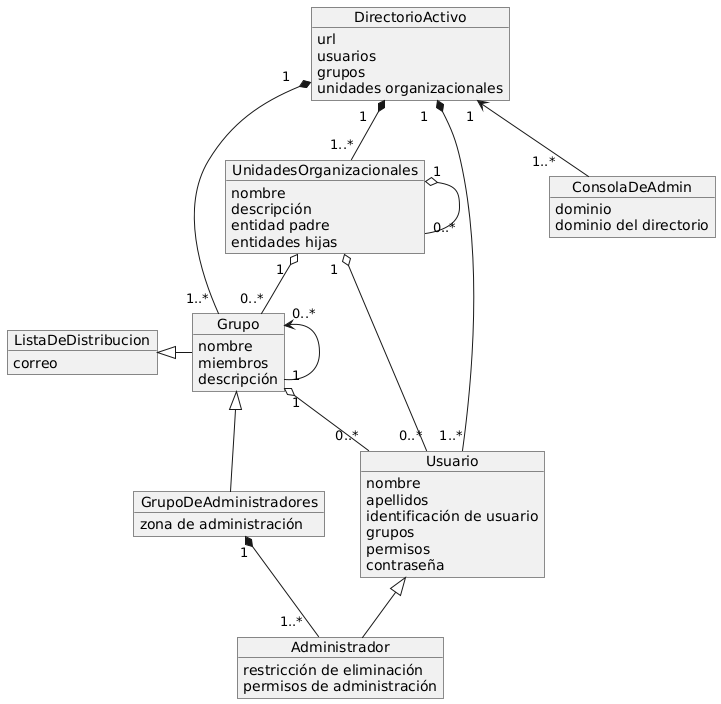
\includegraphics[width=\linewidth]{images/puml/domain-diagram/domain diagram.png}
    \caption{Modelo de dominio del sistema}
    \label{fig:domain-model}
\end{figure}
\subsubsection{Reglas del negocio por patrón}

En el desarrollo de sistemas de información, las reglas de negocio son cruciales, ya que establecen las políticas, restricciones y condiciones que guían el funcionamiento de una organización. Estas reglas resultan fundamentales para asegurar la integridad, consistencia y eficiencia de los procesos en el negocio.

La \autoref{table:bussiness-rules} muestra un resumen de las reglas de negocio identificadas hasta ahora, junto con el patrón que las representa. Esta clasificación facilita la implementación eficiente de dichas reglas en el sistema, garantizando el cumplimiento de los requisitos y expectativas del negocio.


\begin{longtable}{|p{10cm}|l|}
    \caption{Reglas del negocio}
    \label{table:bussiness-rules}                                                                                                                                                                                                                                                                                                          \\
    \hline
    \textbf{Regla}                                                                                                                                                                                                                                                                                                       & \textbf{Patrón} \\
    \hline
    \endfirsthead
    \hline
    Solo si el usuario no existe se puede crear.                                                                                                                                                                                                                                                                         & Precondición    \\ \hline
    Solo si el usuario existe se puede eliminar.                                                                                                                                                                                                                                                                         & Precondición    \\ \hline
    Solo si el usuario existe se puede editar.                                                                                                                                                                                                                                                                           & Precondición    \\ \hline
    Solo si el grupo no existe se puede crear.                                                                                                                                                                                                                                                                           & Precondición    \\ \hline
    Solo si el grupo existe se puede eliminar.                                                                                                                                                                                                                                                                           & Precondición    \\ \hline
    Solo si el grupo existe se puede editar.                                                                                                                                                                                                                                                                             & Precondición    \\ \hline
    Un grupo de tipo lista de distribución tiene: miembros, nombre, descripción y correo electrónico.                                                                                                                                                                                                                    & Estructura      \\ \hline
    Un grupo tiene: miembros, nombre, descripción.                                                                                                                                                                                                                                                                       & Estructura      \\ \hline
    Una unidad organizacional tiene: nombre y descripcion                                                                                                                                                                                                                                                                & Estructura      \\ \hline
    El administrador es responsable de la creación, edición, y eliminación de los usuarios, grupos y unidades organizacionales.                                                                                                                                                                                          & Responsablidad  \\ \hline
    El usuario debe estar autenticado para acceder a las funciones del sistema.                                                                                                                                                                                                                                          & Precondición    \\ \hline
    Solo si no se ha alcanzado el límite de usuarios, el administrador puede crear más usuarios.                                                                                                                                                                                                                         & Precondicion    \\ \hline
    Solo si no se ha alcanzado el límite de grupos, el administrador puede crear más grupos.                                                                                                                                                                                                                             & Precondición    \\ \hline
    Solo si no se ha alcanzado el límite de unidades organizacionales, el administrador puede crear más unidades organizacionales.                                                                                                                                                                                       & Precondición    \\ \hline
    Un usuario tiene nombre, apellidos, nombre de usuario, correo empresarial, correos personales, dirección, carnet de identidad, contraseña, grupos a los que pertenece, permisos, teléfono celular, telefono fijo, telefono de oficina, rol que desempeña dentro de la empresa, quién es su manager y foto de perfil. & Estructura      \\ \hline
    Si el usuario es un objeto crítico, no puede ser eliminado                                                                                                                                                                                                                                                           & Precondición    \\ \hline
    Si el grupo es un objeto crítico, no puede ser eliminado                                                                                                                                                                                                                                                             & Precondición    \\\hline
\end{longtable}


